\documentclass{ctexbeamer}
\usepackage[UTF8]{ctex} % 添加此行确保 listings 支持 UTF8
\usepackage{graphicx}
\usepackage{multicol}

\usefonttheme{serif}
\usefonttheme{professionalfonts}
\definecolor{tyblue}{RGB}{102,204,255}
\usepackage{amsmath}
\usepackage{mathtools}
\usepackage{hyperref}
\usepackage{tikz}
\usetikzlibrary{positioning, shapes.geometric}

\usepackage{listings}
\usepackage{xcolor}

% 自定义代码块样式
\lstset{
    numbers=left,
    numberstyle=\tiny,
    basicstyle=\ttfamily\small, % 推荐加 \small
    keywordstyle=\color{blue!70},
    commentstyle=\color{red!50!green!50!blue!50},
    frame=shadowbox,
    rulesepcolor=\color{red!20!green!20!blue!20},
    escapeinside=``,
    xleftmargin=2em, xrightmargin=2em, aboveskip=1em,
    framexleftmargin=2em,
    language=C,
    extendedchars=true, % 支持扩展字符
    inputencoding=utf8 % 明确指定编码
} 
\usetheme{Antibes}
\usecolortheme{dolphin}

% 自定义 x86-64 汇编语言以改进关键字高亮
\lstdefinelanguage{x86_64}{
  morekeywords={
    mov,add,sub,and,or,xor,not,neg,cmp,test,
    je,jne,jl,jle,jg,jge,jmp,call,ret,
    shr,shl,sar,sal,lea,inc,dec,push,pop,pushq,movq,andl,
    sete,setne,cmove,cmovne,cdqe,cqo,movl,movslq,testl,js,subl,addl,cmpl,
    imull, movsd, addq, cmpq, imulq, xorl,leaq, testq, salq, sarq, cmovns
  },
  sensitive=true,
  morecomment=[l]{;},
  morestring=[b]"
}

\begin{document}

\title{Review: Optimization}
\author{Rainybunny}
\date{\today}
\frame{\titlepage}

\begin{frame}{目录}
  \begin{multicols}{2}
    \tableofcontents
  \end{multicols}
\end{frame}

\AtBeginSection[]{
  \begin{frame} % [shrink=15]
    \begin{multicols}{2}
      \tableofcontents[currentsection]
    \end{multicols}
  \end{frame}
}

\section{Optimization}

\subsection{Code Motion}

\begin{frame}[fragile]{Code Motion}
  \begin{itemize}
    \item Reduce frequency with which computation performed
    \begin{itemize}
      \item If it will always produce same result
      \item Especially moving code out of loop
    \end{itemize}
  \end{itemize}

  \begin{lstlisting}[language=C]
#define N 127
typedef long i64;
typedef unsigned long u64;

i64 rowSum(i64 ary[N][N], int r) {
  i64 res = 0;
  for (int i = 0; i < N; ++i) {
    res += `\color{red}{ary[r]}`[i];
  }
  return res;
}
  \end{lstlisting}

  (所有演示代码: https://godbolt.org/z/4bfnTs6Ev)
\end{frame}

\begin{frame}[fragile,shrink=5]{Code Motion}
  \begin{lstlisting}[language=x86_64]
; -Og -masm=att
rowSum:
    movl    $0, %edx
    movl    $0, %ecx
    jmp     .L2
.L3:
    movslq  %esi, %rax
    imulq   $1016, %rax, %rax
    addq    %rdi, %rax          ; ary[r]
    movslq  %edx, %r8
    addq    (%rax,%r8,8), %rcx  ; res+=ary[r][i]
    addl    $1, %edx
.L2:
    cmpl    $126, %edx
    jle     .L3
    movq    %rcx, %rax
    ret
  \end{lstlisting}
\end{frame}

\begin{frame}[fragile,shrink]{Code Motion}
  \begin{lstlisting}[language=x86_64]
; -O2 -masm=att
rowSum:
    movslq  %esi, %rax
    xorl    %edx, %edx
    imulq   $1016, %rax, %rax
    addq    %rdi, %rax          ; *p=ary[r]
    leaq    1016(%rax), %rcx
.L2:
    addq    (%rax), %rdx        ; res+=p[i]
    addq    $8, %rax
    cmpq    %rcx, %rax
    jne     .L2
    movq    %rdx, %rax
    ret
  \end{lstlisting}
\end{frame}

\subsection{Reduction in Strength}

\begin{frame}{Reduction in Strength}
  \begin{itemize}
    \item Replace costly operation with simpler one
    \begin{itemize}
      \item Shift, add instead of multiply or divide
    \end{itemize}
    \item Recognize sequence of products
  \end{itemize}
\end{frame}

\begin{frame}[fragile,shrink=5]{Reduction in Strength}
  \begin{lstlisting}[language=x86_64]
; -Og -masm=att
rowSum:
    movl    $0, %edx            ; i=0
    movl    $0, %ecx
    jmp     .L2
.L3:
    movslq  %esi, %rax
    imulq   $1016, %rax, %rax
    addq    %rdi, %rax          ; ary[r]
    movslq  %edx, %r8
    addq    (%rax,%r8,8), %rcx  ; res+=ary[r][i]
    addl    $1, %edx            ; ++i
.L2:
    cmpl    $126, %edx          ; i<N
    jle     .L3
    movq    %rcx, %rax
    ret
  \end{lstlisting}
\end{frame}

\begin{frame}[fragile,shrink]{Reduction in Strength}
  \begin{lstlisting}[language=x86_64]
; -O2 -masm=att
rowSum:
    movslq  %esi, %rax
    xorl    %edx, %edx
    imulq   $1016, %rax, %rax
    addq    %rdi, %rax          ; *p=ary[r]
    leaq    1016(%rax), %rcx    ; *q=p+N
.L2:
    addq    (%rax), %rdx        ; res+=*p
    addq    $8, %rax            ; ++p
    cmpq    %rcx, %rax          ; p!=q
    jne     .L2
    movq    %rdx, %rax
    ret
  \end{lstlisting}
\end{frame}

\subsection{Share Common Subexpressions}

\begin{frame}[fragile]{Share Common Subexpressions}
  \begin{itemize}
    \item Reuse portions of expressions
    \item c.f. Code Motion?
  \end{itemize}

  \begin{lstlisting}{language=C}
u64 calc_u(u64 a, u64 b, u64 c, u64 d) {
  return (a + b) * (c + d) + a * c + a * d;
}
  \end{lstlisting}
\end{frame}

\begin{frame}[fragile,shrink]{Share Common Subexpressions}
  \begin{lstlisting}[language=x86_64]
; -Og -masm=att
calc_u:
    leaq    (%rdi,%rsi), %rax ; a+b
    leaq    (%rdx,%rcx), %rsi ; c+d
    imulq   %rsi, %rax        ; (a+b)*(c+d)
    imulq   %rdi, %rdx        ; a*c
    addq    %rdx, %rax        ; res+=a*c
    imulq   %rcx, %rdi        ; b*d
    addq    %rdi, %rax        ; res+=b*d
    ret
  \end{lstlisting}
\end{frame}

\begin{frame}[fragile,shrink]{Share Common Subexpressions}
  \begin{lstlisting}[language=x86_64]
; -O2 -masm=att
calc_u:
    leaq    (%rsi,%rdi,2), %rax ; (2*a)+b
    addq    %rcx, %rdx          ; c+d
    imulq   %rdx, %rax
    ret
  \end{lstlisting}
\end{frame}

\begin{frame}[fragile]{Share Common Subexpressions}
  \qquad 把 \texttt{u64} 换成 \texttt{i64} 会发生什么?

  \begin{lstlisting}[language=C]
i64 calc_i(i64 a, i64 b, i64 c, i64 d) {
  return (a + b) * (c + d) + a * c + a * d;
}
  \end{lstlisting}

  \pause
  \begin{lstlisting}[language=x86_64]
; `\color{red}{-O2}` -masm=att
calc_i:
    leaq    (%rdx,%rcx), %rax
    addq    %rdi, %rsi
    imulq   %rax, %rsi
    imulq   %rdi, %rdx
    imulq   %rcx, %rdi
    addq    %rdx, %rsi
    leaq    (%rsi,%rdi), %rax
    ret
  \end{lstlisting}
\end{frame}

\begin{frame}{Share Common Subexpressions}
  \qquad \texttt{u64} 的运算严格等价于 $\mathbb Z/2^{64}\mathbb Z$, 编译器能够自由地采用结合律, 分配律等化简表达式.
  
  \qquad \texttt{i64} 的运算溢出是\textbf{未定义行为}(Undefined Behavior, UB). 编译器有权假定用户代码不会引入 UB, 但\textbf{不能引入新的 UB 可能}.

  \qquad E.g. \texttt{calc\_i(I64\_MAX, -I64\_MAX + 1, 1, -1)}.
\end{frame}

\subsection{Dead-code Elimination *}

\begin{frame}{Dead-code Elimination *}
  \begin{itemize}
    \item Remove code that does not affect the program results\footnote{https://en.wikipedia.org/wiki/Dead-code\_elimination}
    \begin{itemize}
      \item Shrinking program size
      \item Reducing resource usage such as the number of bytes to be transferred
      \item Allowing the running program to avoid executing irrelevant operations, which reduces its running time
    \end{itemize}
  \end{itemize}
\end{frame}

\begin{frame}[fragile]{Dead-code Elimination *}
  \begin{lstlisting}[language=C]
void squareNonnegative(i64 a) {
  i64 b = a * a;
  if (b < 0) { // gcc: 何意味?
    printf("%lld < 0? WTF?", b);
  } else {
    printf("%lld >= 0 of course.", b);
  }
}
  \end{lstlisting}
\end{frame}

\begin{frame}[fragile]{Dead-code Elimination *}
  \begin{lstlisting}[language=x86_64]
; -O2 -masm=att `\footnote{\texttt{-Og} 行为一样, \texttt{-O0} 会进行正负判断.}`
.LC0:
    .string "%lld >= 0 of course."
squareNonnegative:
    imulq   %rdi, %rdi
    xorl    %eax, %eax
    movq    %rdi, %rsi
    movl    $.LC0, %edi
    jmp     printf
  \end{lstlisting}
\end{frame}

\begin{frame}[fragile,shrink=5]{Dead-code Elimination *}
  \begin{itemize}
    \item \texttt{gcc}: 相信程序员不会写 UB.
    \pause
    \item 程序员: 诶, 我有一计!
  \end{itemize}

  \pause
  \begin{lstlisting}[language=C]
int main() {
  i64 a = (1ll << 61) | (1ll << 1);
  // 刚好溢出到符号位! ohhh!
  squareNonnegative(a);
  return 0;
}
  \end{lstlisting}

  \pause
  \begin{itemize}
    \item \texttt{gcc}: 地铁老人手机.jpg
  \end{itemize}

  \pause
  \begin{lstlisting}
-9223372036854775804 >= 0 of course.
  \end{lstlisting}
\end{frame}

\subsection{Constant Folding *}

\begin{frame}{Constant Folding *}
  \begin{itemize}
    \item Constant folding is the process of recognizing and evaluating constant expressions at compile time rather than computing them at runtime.
  \end{itemize}
\end{frame}

\begin{frame}[fragile,shrink=10]{Constant Folding *}
  \begin{lstlisting}[language=C++]
// -std=c++11
constexpr u64 fibo(u64 n) {
  return n <= 1 ? 1 : fibo(n - 1) + fibo(n - 2);
}

int main() {
    printf("%lld\n", fibo(35));
    return 0;
}
  \end{lstlisting}

  \pause
  \qquad 你说得对\dots
  \begin{lstlisting}[language=x86_64]
; -O2 -masm=att
    ; ...
    movl    $14930352, %esi
    ; ...
  \end{lstlisting}

  \pause
  但是编译了 16603ms (编译时递归硬算出 \texttt{fibo(35)}).
\end{frame}

\subsection{Induction Variable *}

\begin{frame}{Induction Variable *}
  \begin{itemize}
    \item An induction variable is a variable that gets increased or decreased by a fixed amount on every iteration of a loop or is a linear function of another induction variable.
  \end{itemize}
\end{frame}

\section{Optimization Blockers}

\subsection{Procedure Calls}

\begin{frame}[fragile,shrink]{Procedure Calls}
  \begin{lstlisting}[language=C]
__attribute__((noinline))
i64 length(const char* str) {
    i64 res = 0;
    while (str[res] > 0) ++res; // intended
    return res;
}

void toLower(char* __restrict__ str) {
    for (i64 i = 0; i < length(str); ++i) {
        if ('A' <= str[i] && str[i] <= 'Z') {
            str[i] += 'a' - 'A';
        }
    }
}
  \end{lstlisting}

  \pause
  \begin{itemize}
    \item Compiler treats procedure call as a black box
  \end{itemize}
\end{frame}

\begin{frame}[fragile,shrink]{Procedure Calls}
  \begin{itemize}
    \item \texttt{inline} 一定能拯救吗?
  \end{itemize}

  \begin{lstlisting}[language=C]
__attribute__((always_inline)) inline
i64 length(const char* str) {
    i64 res = 0;
    while (str[res] > 0) ++res;
    return res;
}
  \end{lstlisting}

  \pause
  \begin{itemize}
    \item 不一定.
    \pause
    \item \texttt{length} 本身不是关于形参 \texttt{str} 的纯函数, 它还依赖于 \texttt{str} 指向的一段内存. 而 \texttt{toLower} 中的确会修改 \texttt{str} 指向的内存, 编译器未能发现这些修改不会导致 \texttt{length} 的结果改变.
  \end{itemize}
\end{frame}

\subsection{Memory Aliasing}

\begin{frame}[fragile,shrink=5]{Memory Aliasing}
  \begin{lstlisting}[language=C]
void i64cpy(i64* dst, const i64* src, u64 n) {
    for (u64 i = 0; i < n; ++i) {
        dst[i] = src[i];
    }
}
  \end{lstlisting}

  \begin{itemize}
    \item 程序员: 总不能有人调用 \texttt{i64cpy(src, src + 1, n)} 吧?
    \pause
    \item \texttt{gcc}: 总有神人会调用 \texttt{i64cpy(src, src + 1, n)} 的...
  \end{itemize}

  \begin{lstlisting}[language=x86_64]
; -O2 -masm=att
i64cpy(long*, long const*, unsigned long):
    testq   %rdx, %rdx
    je      .L25
    xorl    %eax, %eax
.L27:
    movq    (%rsi,%rax,8), %rcx
    movq    %rcx, (%rdi,%rax,8)
    addq    $1, %rax
    cmpq    %rax, %rdx
    jne     .L27
.L25:
    ret
  \end{lstlisting}
\end{frame}

\begin{frame}[fragile,shrink=5]{Memory Aliasing}
  \begin{itemize}
    \item 手动消除 aliasing: 用变量暂存计算结果, 减少内存写回;
    \item 相信现代编译器的指针分析.
    \pause
    \item 直接告诉编译器!
  \end{itemize}

  \begin{lstlisting}[language=C]
void i64cpy_restr(i64* __restrict__ dst,
    const i64* __restrict__ src, u64 n) {
    for (u64 i = 0; i < n; ++i) {
        dst[i] = src[i];
    }
}
  \end{lstlisting}

  \begin{itemize}
    \item 程序员: 放心吧, 没有神人.
    \pause
    \item \texttt{gcc}: 那还说啥? 我看懂了!
  \end{itemize}

  \begin{lstlisting}[language=x86_64]
; -O2 -masm=att
i64cpy_restr(long*, long const*, unsigned long):
    testq   %rdx, %rdx
    je      .L32
    salq    $3, %rdx
    jmp     memcpy
.L32:
    ret
  \end{lstlisting}
\end{frame}

\subsection{Bonus: C++ Attribute *}

\begin{frame}{Bonus: C++ Attribute *}
  \begin{itemize}
    \item 我知道 \texttt{exit()} 不会返回, 我知道 \texttt{int count} 其实一定是非负整数, 我知道 \texttt{isprime(n)} 很可能是 \texttt{false}...
    \pause
    \item \texttt{gcc}: tell me!
    \item \texttt{[[noreturn]]}, \texttt{[[assume(...)]]}, \texttt{[[unlikely]]}, \dots\footnote{https://en.cppreference.com/w/cpp/language/attributes.html}
    \pause
    \item \textbf{若 attribute 被违背, 行为未定义.}
  \end{itemize}
\end{frame}

\begin{frame}[fragile, shrink=5]{Bonus: C++ Attribute *}
  \begin{lstlisting}[language=C]
/* https://zhuanlan.zhihu.com/p/663893518 */
i64 div128(i64 x) {
    return x / 128;
}

// -std=c++23
i64 div128_assume(i64 x) {
    [[assume(x >= 0)]];
    return x / 128;
}
  \end{lstlisting}

  \begin{lstlisting}[language=x86_64]
; -O2 -masm=att -std=c++23
div128(long):
    testq   %rdi, %rdi
    leaq    127(%rdi), %rax
    cmovns  %rdi, %rax
    sarq    $7, %rax
    ret
div128_assume(long):
    movq    %rdi, %rax
    sarq    $7, %rax
    ret
  \end{lstlisting}
\end{frame}

\section{Instruction-Level Parallelism}

\subsection{Modern CPU Design}

\begin{frame}{Mordern CPU Design}
  \begin{itemize}
    \item Superscalar Processor
    \pause
    \item Multiple Functional Units
    \pause
    \item Pipelined Functional Units
    \begin{itemize}
      \item Latency Bound
      \item Throughput Bound
    \end{itemize}
  \end{itemize}
\end{frame}

\subsection{Unrolling}

\begin{frame}[fragile]{Unrolling: Key Ideas}
  \begin{lstlisting}[language=C]
void combine4(vec_ptr v, data_t *dest) {
    long i, length = vec_length(v);
    data_t *d = get_vec_start(v);
    data_t t = IDENT;
    for (i = 0; i < length; i++)
        t = t OP d[i];
    *dest = t;
}
  \end{lstlisting}

  \begin{itemize}
    \item \textbf{连续且无数据依赖的指令}更能充分发挥 CPU 性能, 但是:
    \begin{itemize}
      \item \texttt{OP} 是结合的, 而 \texttt{combine4 = foldl (OP) IDENT};
      \item \texttt{OP} 是交换的, 而 \texttt{combine4} 只用单变量累加.
    \end{itemize}
  \end{itemize}
\end{frame}

\begin{frame}[fragile,shrink=5]{Unrolling 2x1}
  \begin{lstlisting}[language=C]
void combine_2x1(vec_ptr v, data_t *dest) {
    long length = vec_length(v);
    long limit = length-1;
    data_t *d = get_vec_start(v);
    data_t x = IDENT;
    long i;
    for (i = 0; i < limit; i+=2) {
        x = (x OP d[i]) OP d[i+1];
    }
    for (; i < length; i++) {
        x = x OP d[i];
    }
    *dest = x;
}
  \end{lstlisting}

  \begin{itemize}
    \item 相比原版, \texttt{int add} 得到部分优化.
  \end{itemize}
\end{frame}

\begin{frame}[fragile,shrink=5]{Unrolling 2x1a: Reassociation}
  \begin{lstlisting}[language=C]
void combine_2x1a(vec_ptr v, data_t *dest) {
    long length = vec_length(v);
    long limit = length-1;
    data_t *d = get_vec_start(v);
    data_t x = IDENT;
    long i;
    for (i = 0; i < limit; i+=2) {
        `\color{red}x = x OP (d[i] OP d[i+1]);`
    }
    for (; i < length; i++) {
        x = x OP d[i];
    }
    *dest = x;
}
  \end{lstlisting}

  \begin{itemize}
    \item 相比 2x1, 其他的 \texttt{CPE} 几乎减半.
  \end{itemize}
\end{frame}

\begin{frame}[fragile,shrink=5]{Unrolling 2x2: Separate Accumulator}
  \begin{lstlisting}[language=C]
void combine_2x2(vec_ptr v, data_t *dest) {
    long length = vec_length(v);
    long limit = length-1;
    data_t *d = get_vec_start(v);
    data_t x0 = IDENT;
    data_t x1 = IDENT;
    long i;
    for (i = 0; i < limit; i+=2) {
        x0 = x0 OP d[i];
        x1 = x1 OP d[i+1];
    }
    for (; i < length; i++) {
       x0 = x0 OP d[i];
    }
    *dest = x0 OP x1;
}
  \end{lstlisting}

  \begin{itemize}
    \item 相比 2x1a, \texttt{int add} 得到部分优化.
  \end{itemize}
\end{frame}

\begin{frame}{Unrolling: Result Table}
  \begin{center}
    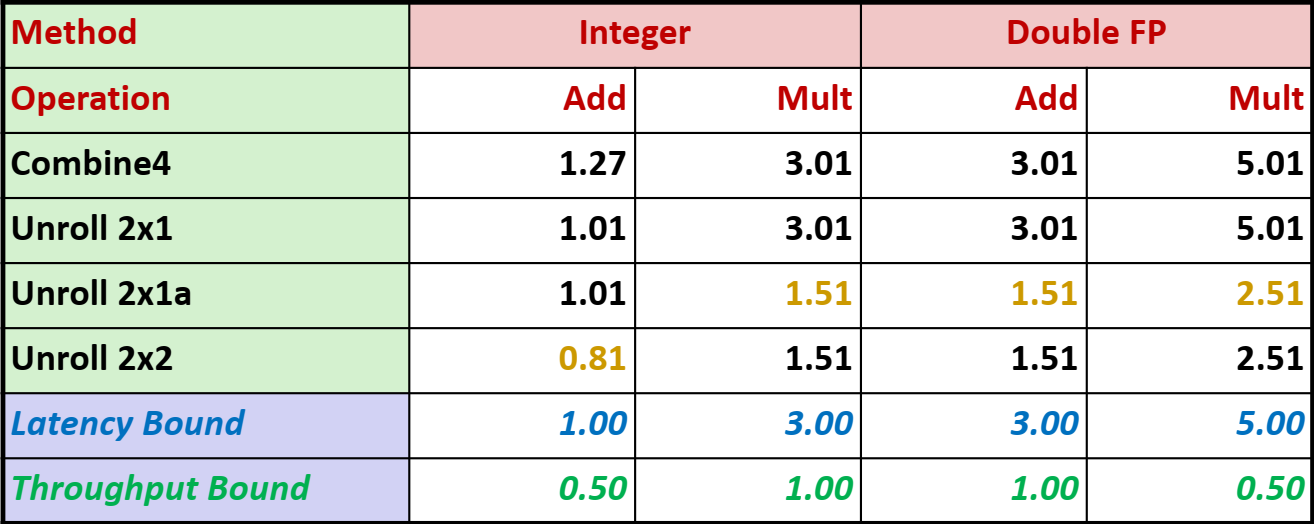
\includegraphics[width=\textwidth]{./unroll-perform.png}
  \end{center}

  \pause
  \begin{itemize}
    \item 进一步优化: 增大展开路数, 激发 functional units 流水化.
    \item 思考:
    \begin{itemize}
      \item 为什么刚刚的 unrolling 几乎没有激发流水化?
      \pause
      \item 从理论上分析, 几路展开能让 \texttt{double mult} 贴近 throughput bound?
            (2 fp pipelined mult units, latency = 5; 2 fp load units)
    \end{itemize}
  \end{itemize}
\end{frame}

\begin{frame}{Unrolling: Demostration}
  \begin{itemize}
    \item CPU: \texttt{AMD Ryzen 9 8945HS w/ Radeon 780M Graphics}
    \item gcc: \texttt{gcc version 11.4.0 (Ubuntu 11.4.0-1ubuntu1~22.04.2)}
    \item target: \texttt{x86\_64-linux-gnu}
    \item option: \texttt{-Og -masm=att -std=c11}
    \item test code and script: \texttt{https://paste.ubuntu.com/p/kmP4GK7Rg5}
  \end{itemize}
\end{frame}

\begin{frame}[plain]
  % \vspace{0.4\textheight}
  \begin{center}
    \Huge\color{tyblue}\bfseries Thanks!
  \end{center}
\end{frame}

\end{document}
